\documentclass[signature=data]{physicsreport}

%%
%% User settings
%%

\classno{}
\stuno{}
\groupno{}
\stuname{}
\expdate{\expdatefmt\today}
\expname{示波器实验}

%%
%% Document body
%%

\begin{document}
% First page
% Some titles and personal information are defined in ``\maketitle''.
\maketitle
\subsection{讨论题}

\newpage
\subsection{讨论题}
\subsection{讨论题}

\newpage
\subsection{讨论题}

\newpage

% Data process and others
\subsection{实验结论及现象分析}

\begin{figure}[htbp]
    \centering
    \begin{minipage}[t]{0.3\textwidth}
        \centering
        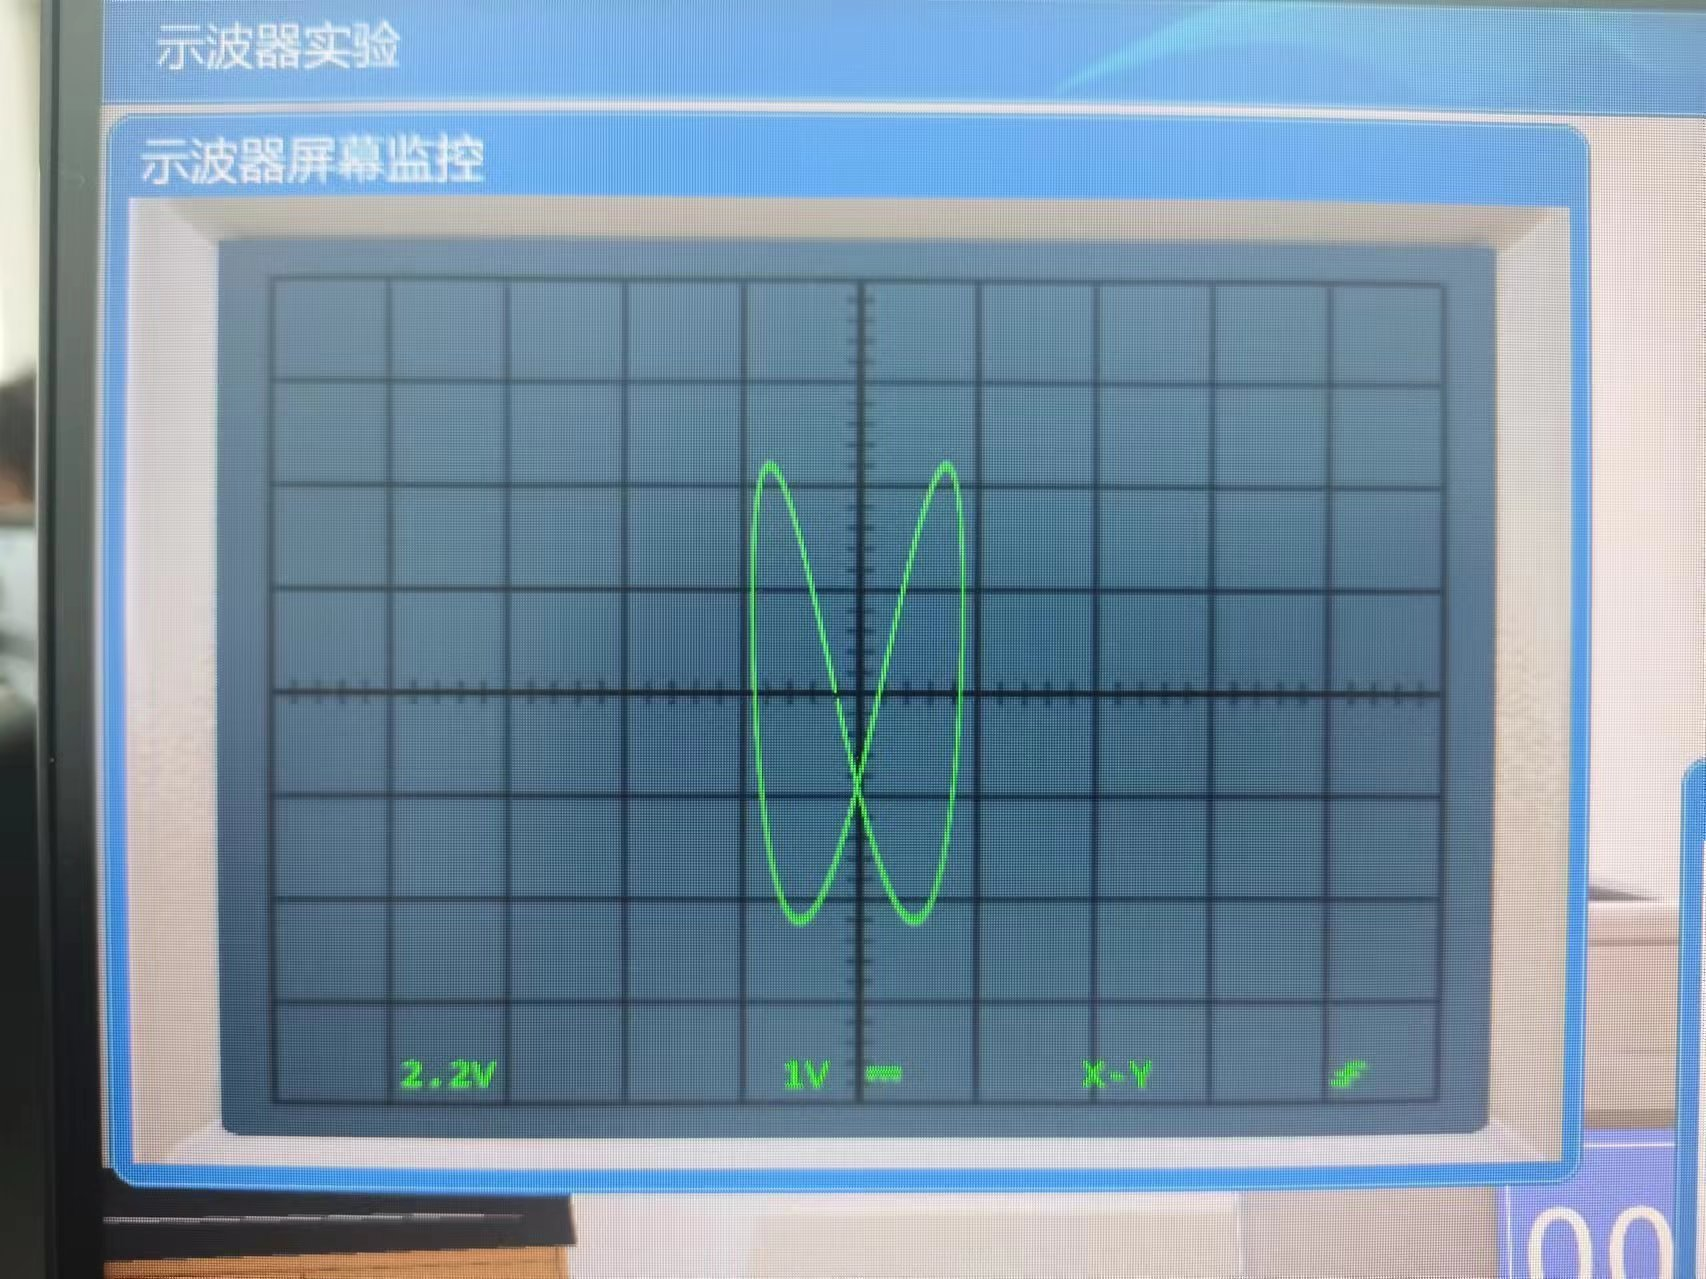
\includegraphics[width=\textwidth]{images/lab6/image1.jpg}
        \caption{}
    \end{minipage}
    \hfill
    \begin{minipage}[t]{0.3\textwidth}
        \centering
        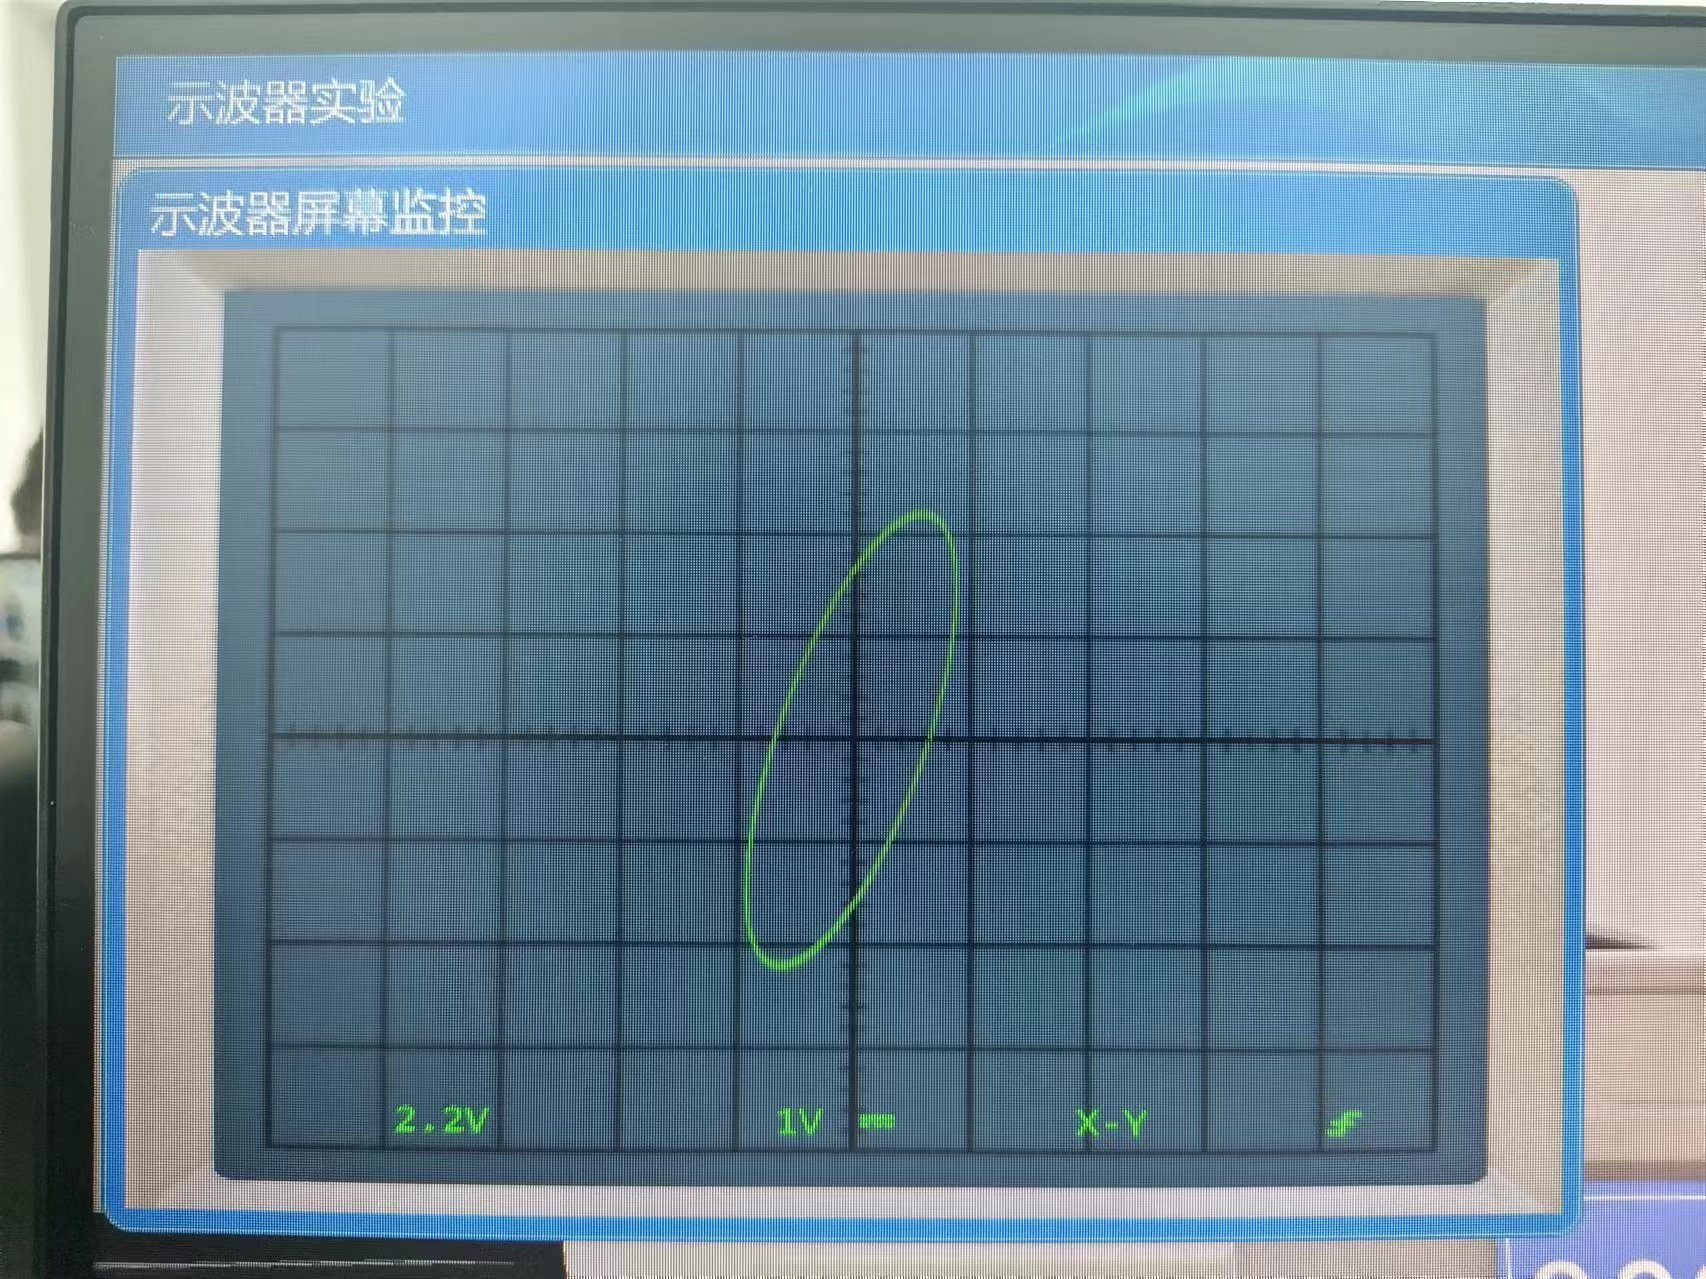
\includegraphics[width=\textwidth]{images/lab6/image2.jpg}
        \caption{}
    \end{minipage}
    \hfill
    \begin{minipage}[t]{0.3\textwidth}
        \centering
        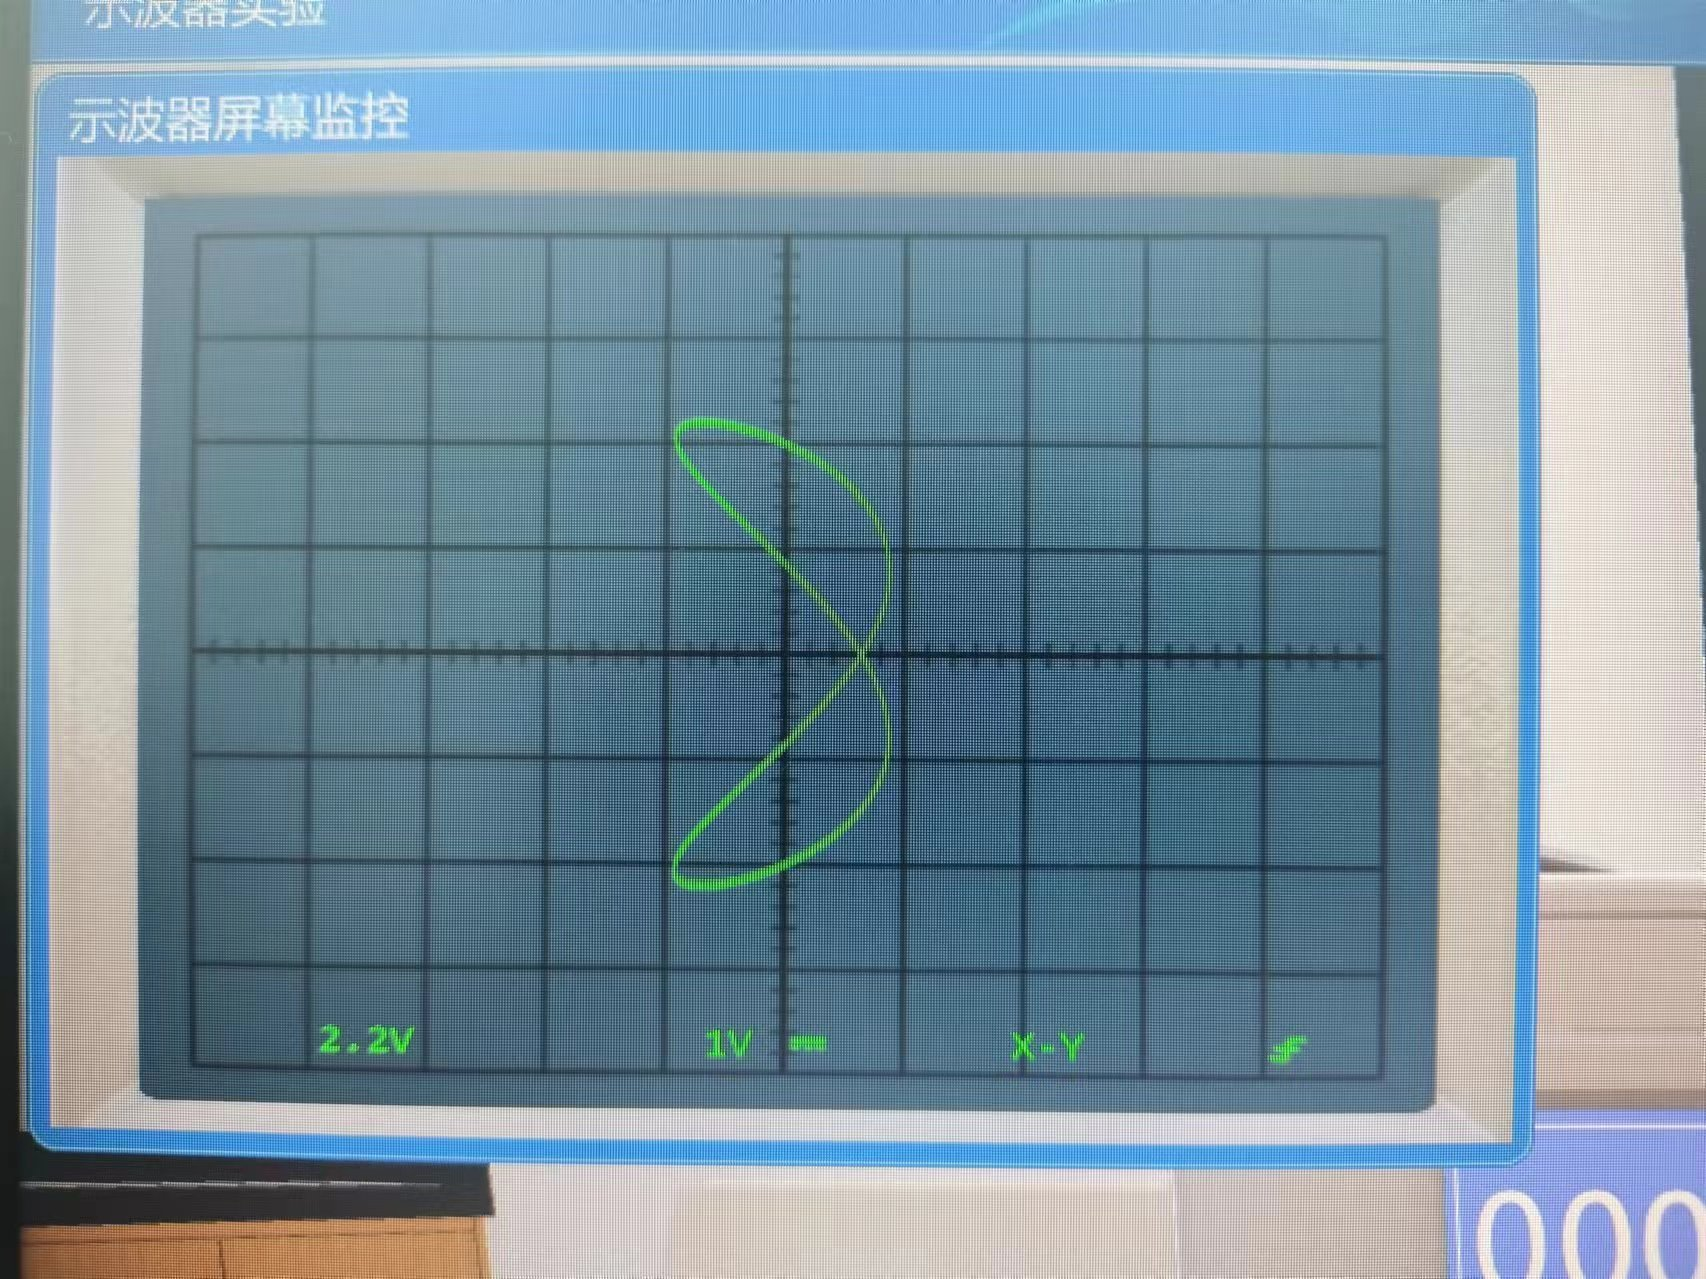
\includegraphics[width=\textwidth]{images/lab6/image3.jpg}
        \caption{}
    \end{minipage}

    \caption*{李萨如图形}
\end{figure}

\begin{itemize}
    \item 实验结论:示波器是一种重要的电子测量仪器,能够将电信号转化为可视化的波形图。在观察和测量电子信号方面,示波器通过捕捉微弱信号和细微变化,为复杂信号的分析提供了新的思路和方法。这次实验,我掌握了示波器的基本操作和使用方法,熟悉了示波器在电路实验中的应用,加深了对信号之间的相位差和频率关系的理解。
    \vspace{1em}
    \item 现象分析:李萨如图形的形成原理基于两个正弦信号之间的相互叠加。当这两个信号的频率不同且它们的相位差随时间变化时,相互叠加的结果就会形成复杂的运动轨迹,从而在示波器屏幕上呈现出各种各样的图案。
    
    当两个信号的频率相等且相位差为零时,产生的李萨如图形是一个椭圆;当相位差不为零时,椭圆的形状将发生旋转。当两个信号的频率不同但它们之间存在简单的整数倍关系时,比如1:2,2:3等,产生的图形则会是一些闭合的曲线,比如椭圆、圆或者直线。而当两个信号的频率无法用简单整数关系表示时,将会产生一些复杂而不规则的图形。
\end{itemize}

\vspace{3em}

\subsection{讨论题}
假定在示波器的y轴输入一个正弦电压,所用的水平扫描频率为120Hz,在荧光屏上出现三个稳定的正弦波形,那么输入信号的频率是多少?这是否是测量信号频率的好方法?为什么?

\vspace{2em}

示波器的水平扫描频率为120Hz,即示波器屏幕上每秒钟出现120个波形。由于屏幕上出现了三个稳定的正弦波形,说明输入信号的频率是水平扫描频率的三倍,即$120\times3=360$Hz。

不是一个好方法。示波器观察到的三个正弦波形不是直接的信号频率,是一种间接关系。 输入信号源的稳定性和准确性会对测量结果造成影响。示波器的水平扫描频率与输入信号的频率存在整数倍关系时,会使得实际观察到的波形数量与输入信号的频率并不直接相关,造成误差。
\end{document}